\documentclass[11pt,a4paper]{article}
\usepackage[final]{acl}
\usepackage{fontspec}
\usepackage{polyglossia}
\setmainlanguage{vietnamese}
\setmainfont{Times New Roman}
\usepackage{graphicx}
\usepackage{booktabs}
\title{Milestone: So sánh Vision Transformer và CNN trên CIFAR-10}
\author{Lan Anh: \underline{\hspace{1cm}} \\ MSSV: \underline{\hspace{1.6cm}}
\And Hiền: \underline{\hspace{1cm}} \\ MSSV: \underline{\hspace{1.6cm}}
\And Minh: \underline{\hspace{1cm}} \\ MSSV: \underline{\hspace{1.6cm}}}
\begin{document}
\maketitle
\begin{abstract}
Nhóm so sánh Vision Transformer tự cài với ResNet có số tham số tương đương khi thay đổi lượng dữ liệu huấn luyện trên CIFAR-10. Đến mốc báo cáo, nhóm có sáu lượt validation ở ba tỷ lệ dữ liệu với một cặp seed và ngân sách 100 epoch. ResNet đạt 74,24\%, 88,40\%, 91,80\%; ViT đạt 52,16\%, 67,66\%, 75,90\% theo tỷ lệ 10\%, 50\%, 100\%. Hai mô hình dùng cùng manifest và preprocessing. Báo cáo trình bày tiến độ, các kết quả hiện có, giới hạn và phần việc còn lại. Hai seed bổ sung và đánh giá test cuối đang chờ thực hiện.
\end{abstract}

\section{Bài toán và phương pháp}
Đầu vào là ảnh RGB $32\times32$; đầu ra là logits 10 lớp, nhãn dự đoán và phân phối xác suất. Câu hỏi nghiên cứu là chênh lệch accuracy giữa ViT và CNN thay đổi thế nào khi tăng lượng dữ liệu.

Lan Anh xây ViT dựa trên \citet{dosovitskiy2020image}: patch $4\times4$, 64 patch và một CLS token, embedding 96 chiều, bốn encoder block, bốn head, MLP ratio 1,5 và dropout 0,1. Các khối attention, residual và positional embedding được cài bằng PyTorch. Mô hình có 274.282 tham số trainable.

Minh xây CIFAR-style ResNet dựa trên \citet{he2015deep}, width 16, ba basic block mỗi stage, projection shortcut và classifier 10 lớp. Mô hình có 272.474 tham số, chênh 0,66\% so với ViT theo mẫu số ResNet. Cả hai khởi tạo từ đầu.

\section{Dữ liệu và thiết lập}
CIFAR-10 \citep{krizhevsky2009learning} được chia phân tầng 45.000 train và 5.000 validation từ tập train gốc. Tập test 10.000 ảnh được giữ riêng. Các tập con 4.500, 22.500, 45.000 ảnh lồng nhau và cân bằng lớp. Hai mô hình dùng cùng chỉ số ở từng tỷ lệ; split seed 2026 và train seed 42.

Train dùng random crop padding 4 và random horizontal flip, sau đó chuyển tensor và chuẩn hóa. Validation chỉ chuyển tensor và chuẩn hóa với cùng hằng số. Các manifest được kiểm tra không giao nhau và lưu SHA-256.

Sáu lượt chính dùng batch 128, 100 epoch, cosine annealing theo epoch. ViT dùng AdamW với LR 0,0003 và weight decay 0,05. ResNet dùng SGD với LR 0,05, momentum 0,9 và weight decay 0,0005. Chọn best.pt theo validation accuracy cao nhất; khi hòa giữ epoch sớm hơn. TensorBoard và CSV ghi diễn biến từng epoch.

\section{Kết quả và phân tích sơ bộ}
\begin{table}[t]
\centering
\begin{tabular}{lrrr}
\toprule
Train & ViT & ResNet & Chênh lệch \\
\midrule
10\% & 52,16 & 74,24 & 22,08 \\
50\% & 67,66 & 88,40 & 20,74 \\
100\% & 75,90 & 91,80 & 15,90 \\
\bottomrule
\end{tabular}
\caption{Top-1 validation accuracy (\%). Chênh lệch ResNet trừ ViT, tính bằng điểm phần trăm. Mỗi cấu hình có một seed.}
\label{tab:results}
\end{table}

Bảng~\ref{tab:results} cho thấy accuracy tăng theo lượng ảnh ở cả hai mô hình. Chênh lệch giảm từ 22,08 xuống 15,90 điểm phần trăm. Các lượt được chọn theo cùng tiêu chí validation. Tổng số bước cập nhật lần lượt 3.600, 17.600 và 35.200 cho mỗi mô hình ở ba tỷ lệ.

Tổng thời gian train GPU của ResNet lần lượt 104,29; 498,78; 1.001,87 giây, ViT là 96,41; 467,54; 900,67 giây theo log của các lượt đã chạy. Chi phí này phụ thuộc máy và thời điểm thực thi. Khởi động, validation và ghi checkpoint tạo thêm chi phí ngoài thời gian train được cộng trong log.

CNN có locality và weight sharing, còn ViT dùng attention toàn cục và positional embedding. Kết quả hiện có phù hợp với việc khảo sát các khác biệt này, nhưng tác động riêng của inductive bias chưa được tách khỏi optimizer, regularization và quá trình tối ưu. Cùng 100 epoch khi tăng lượng ảnh cũng làm tăng số bước cập nhật.

\begin{figure}[t]
\centering
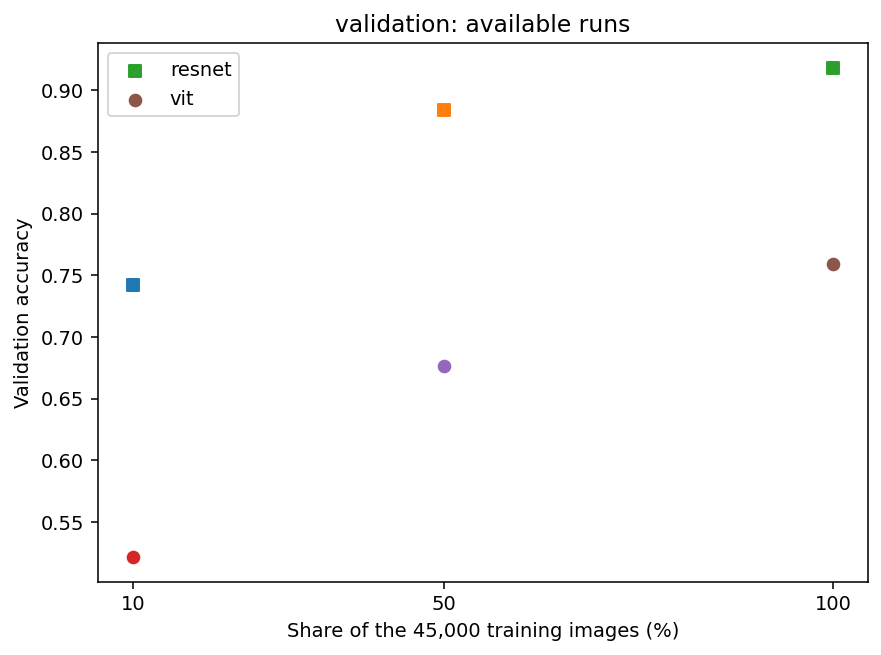
\includegraphics[width=\linewidth]{../results/team_week2/visualizations/accuracy_data.png}
\caption{Validation ở ba tỷ lệ, một seed. Hình được tạo từ sáu checkpoint P0 trên GPU.}
\end{figure}

\section{Tiến độ và bằng chứng}
Đã có sáu learning curve, sáu confusion matrix và ba attention map thử. Attention hiện dùng ảnh đúng và sai đầu tiên theo thứ tự manifest, lấy CLS tới patch ở block cuối, trung bình bốn head, ánh xạ lưới $8\times8$ lên ảnh $32\times32$. Attention cần được diễn giải như quan sát trực quan và đối chiếu với nhãn dự đoán.

Hiền đã đối chiếu bảng CSV với 100 epoch log của từng run, số ảnh, hash manifest, số bước và epoch tốt nhất. Trong bản checkout hiện tại, các ZIP và checkpoint P0 còn chờ chuyển từ máy Minh. Bằng chứng evaluator CUDA khớp trainer do Minh bàn giao được giữ trong results/team\_week2/checks.json. ViT 10\% khi đánh giá CPU chênh một ảnh so với CUDA, nên đối chiếu lại dùng thiết bị đã ghi trong run.

Công cụ tuần 3 cập nhật ma trận 18 lượt, xuất bảng từng seed và mean/std mẫu. Hiện có 6/18 lượt; std mẫu được ghi N/A cho mỗi cấu hình một seed. Quy tắc ảnh cố định mới chọn hai chỉ số CIFAR nhỏ nhất mỗi lớp thuộc validation, độc lập với kết quả dự đoán. Công cụ đã chuẩn bị ghép lỗi theo cùng ảnh thành bốn nhóm: cả hai đúng, chỉ ViT sai, chỉ ResNet sai, cả hai sai. Xuất hình ghép lỗi và attention nhiều lớp cần các checkpoint.

\section{Khó khăn và kế hoạch}
Hai seed còn lại dùng các cặp (split, train) là (2027,43) và (2028,44), tương ứng 12 lượt bổ sung. Hiền cập nhật bảng sau khi nhận log/config và kiểm tra manifest, recipe trước khi tổng hợp. Giữ cùng recipe qua các tỷ lệ.

Ưu tiên tiếp theo là nhận sáu gói run, kiểm tra checksum, xuất attention trên bộ ảnh cố định và ghép lỗi trên cùng validation. Sau khi đủ seed, nhóm tính mean và độ lệch chuẩn mẫu với $ddof=1$. Lan Anh tiếp tục ablation positional embedding, Minh chuẩn bị Swin như phần mở rộng \citep{liu2021swin}. Nhóm khóa phương pháp và checkpoint trước đánh giá test cuối.

\section*{Giới hạn và đóng góp}
Phân tích hiện có một seed và chỉ dùng CIFAR-10. Chưa có thống kê biến thiên seed hoặc kết quả test. Chênh lệch recipe và số bước giới hạn kết luận về nguyên nhân.

Lan Anh phụ trách mô hình ViT, mã và phần viết kiến trúc. Minh phụ trách mô hình ResNet, trainer và tái lập. Hiền phụ trách dữ liệu, mã đánh giá, đối chiếu, bảng/hình, công cụ phân tích và ghép milestone. Mã và bản thảo có hỗ trợ AI; nhóm cần đọc duyệt và chịu trách nhiệm trước khi nộp. Họ tên/MSSV được để trống theo yêu cầu. Bản này chờ nhóm duyệt và nộp theo hạn môn.
\bibliography{references}
\end{document}
